% v2-acmsmall-sample.tex, dated March 6 2012
% This is a sample file for ACM small trim journals
%
% Compilation using 'acmsmall.cls' - version 1.3 (March 2012), Aptara Inc.
% (c) 2010 Association for Computing Machinery (ACM)
%
% Questions/Suggestions/Feedback should be addressed to => "acmtexsupport@aptaracorp.com".
% Users can also go through the FAQs available on the journal's submission webpage.
%
% Steps to compile: latex, bibtex, latex latex
%
% For tracking purposes => this is v1.3 - March 2012

\documentclass[prodmode,acmtecs]{acmsmall} % Aptara syntax

\usepackage{caption}
\usepackage{subfig}
\captionsetup[subfigure]{margin=5pt}

% Metadata Information
% \acmVolume{9}
% \acmNumber{4}
% \acmArticle{39}
% \acmYear{2010}
% \acmMonth{3}

% Copyright
%\setcopyright{acmcopyright}
%\setcopyright{acmlicensed}
%\setcopyright{rightsretained}
%\setcopyright{usgov}
%\setcopyright{usgovmixed}
%\setcopyright{cagov}
%\setcopyright{cagovmixed}
%
% % DOI
% \doi{0000001.0000001}
%
% %ISSN
% \issn{1234-56789}

% Document starts
\begin{document}

% Page heads
\markboth{B. Berger et al.}{Computational biology in the 21st century: Algorithms that scale}

% Title portion
\title{Computational biology in the 21st century: Algorithms that scale}
\author{BONNIE BERGER
\affil{Massachusetts Institute of Technology}
NOAH M. DANIELS
\affil{Massachusetts Institute of Technology}
Y. WILLIAM YU
\affil{Massachusetts Institute of Technology}}


\begin{abstract}
Throughout all areas of data science, scientists are being confronted by a
veritable explosion of available data. In many fields, this increase is
exponential in nature, even outpacing Moore's and Kryder's laws on the
respective doublings of transistors on a chip and long-term data storage
density. As such, the challenges posed by the massive influx of data cannot
be solved by waiting for faster and larger capacity computers, but require
instead the development of data structures and representations that exploit
and simplify complexity in the dataset. In this Review, we
survey the biological data landscape, with a focus on how taking advantage
of the structure of massive biological data enables the design of algorithms
that scale sublinearly in large-scale genomics, personal genomics and
chemogenomics.
\end{abstract}


%
% The code below should be generated by the tool at
% http://dl.acm.org/ccs.cfm
% Please copy and paste the code instead of the example below. 
%
% \begin{CCSXML}
% <ccs2012>
%  <concept>
%   <concept_id>10010520.10010553.10010562</concept_id>
%   <concept_desc>Computer systems organization~Embedded systems</concept_desc>
%   <concept_significance>500</concept_significance>
%  </concept>
%  <concept>
%   <concept_id>10010520.10010575.10010755</concept_id>
%   <concept_desc>Computer systems organization~Redundancy</concept_desc>
%   <concept_significance>300</concept_significance>
%  </concept>
%  <concept>
%   <concept_id>10010520.10010553.10010554</concept_id>
%   <concept_desc>Computer systems organization~Robotics</concept_desc>
%   <concept_significance>100</concept_significance>
%  </concept>
%  <concept>
%   <concept_id>10003033.10003083.10003095</concept_id>
%   <concept_desc>Networks~Network reliability</concept_desc>
%   <concept_significance>100</concept_significance>
%  </concept>
% </ccs2012>
% \end{CCSXML}
%
% \ccsdesc[500]{Computer systems organization~Embedded systems}
% \ccsdesc[300]{Computer systems organization~Redundancy}
% \ccsdesc{Computer systems organization~Robotics}
% \ccsdesc[100]{Networks~Network reliability}

%
% End generated code
%

% We no longer use \terms command
%\terms{Design, Algorithms, Performance}

\keywords{computational biology, database search, metagenomics, chemogenomics}

\acmformat{Bonnie Berger, Noah M. Daniels,
and Y. William Yu, 2015. Computational biology in the 21st century: Algorithms that scale.}
% At a minimum you need to supply the author names, year and a title.
% IMPORTANT:
% Full first names whenever they are known, surname last, followed by a period.
% In the case of two authors, 'and' is placed between them.
% In the case of three or more authors, the serial comma is used, that is, all author names
% except the last one but including the penultimate author's name are followed by a comma,
% and then 'and' is placed before the final author's name.
% If only first and middle initials are known, then each initial
% is followed by a period and they are separated by a space.
% The remaining information (journal title, volume, article number, date, etc.) is 'auto-generated'.

\begin{bottomstuff}
This work is supported by the National Institutes of Health, under
grant GM108348.
% This work is supported by the National Science Foundation, under
% grant CNS-0435060, grant CCR-0325197 and grant EN-CS-0329609.
%
% Author's addresses: G. Zhou, Computer Science Department,
% College of William and Mary; Y. Wu  {and} J. A. Stankovic,
% Computer Science Department, University of Virginia; T. Yan,
% Eaton Innovation Center; T. He, Computer Science Department,
% University of Minnesota; C. Huang, Google; T. F. Abdelzaher,
% (Current address) NASA Ames Research Center, Moffett Field, California 94035.
\end{bottomstuff}

\maketitle


\section{Introduction}

Computational biologists answer biological and biomedical 
questions by using computation in support of---or in place of---laboratory 
procedures, in hopes of obtaining more accurate answers at a greatly reduced 
cost.
The past two decades have seen unprecedented technological progress with regard
to generating biological data; next-generation sequencing, mass spectroscopy,
microarrays, nuclear magnetic resonance spectroscopy, and other high-throughput 
approaches have led to an explosion of data.
However, this explosion of data is a mixed blessing.
On the one hand, the scale and scope of data should allow new insights into
genetic and infectious diseases, cancer, basic biology, and even human migration
patterns.
On the other hand, researchers are generating datasets so massive that it has 
become difficult to analyze them to discover patterns that give clues to the 
underlying biological processes.

Certainly, computers are getting faster and more economical; the amount of 
processing available per dollar of compute hardware is more or less doubling 
every year or two; a similar claim can be made about storage capacity 
(Figure~\ref{fig:growth}).
In 2002, when the first human genome was sequenced, the growth in computing 
power was still matching the growth rate of genomic data.
However, the sequencing technology used for the Human Genome Project--Sanger
sequencing--was supplanted around 2004, with the advent of what is now known as 
next-generation sequencing.
The material costs to sequence a genome have plummeted in the past
decade, to the point where a whole human genome can be sequenced for less than
one thousand U.S. Dollars.
As a result, the amount of genomic data available to 
researchers is increasing by a factor of ten every year.

\begin{figure}[htb!]
\centering
\subfloat[Growth of genomic sequence data (orange) as compared with the combined power of the top-500 supercomputer list (blue); y-axis is logarithmic]{
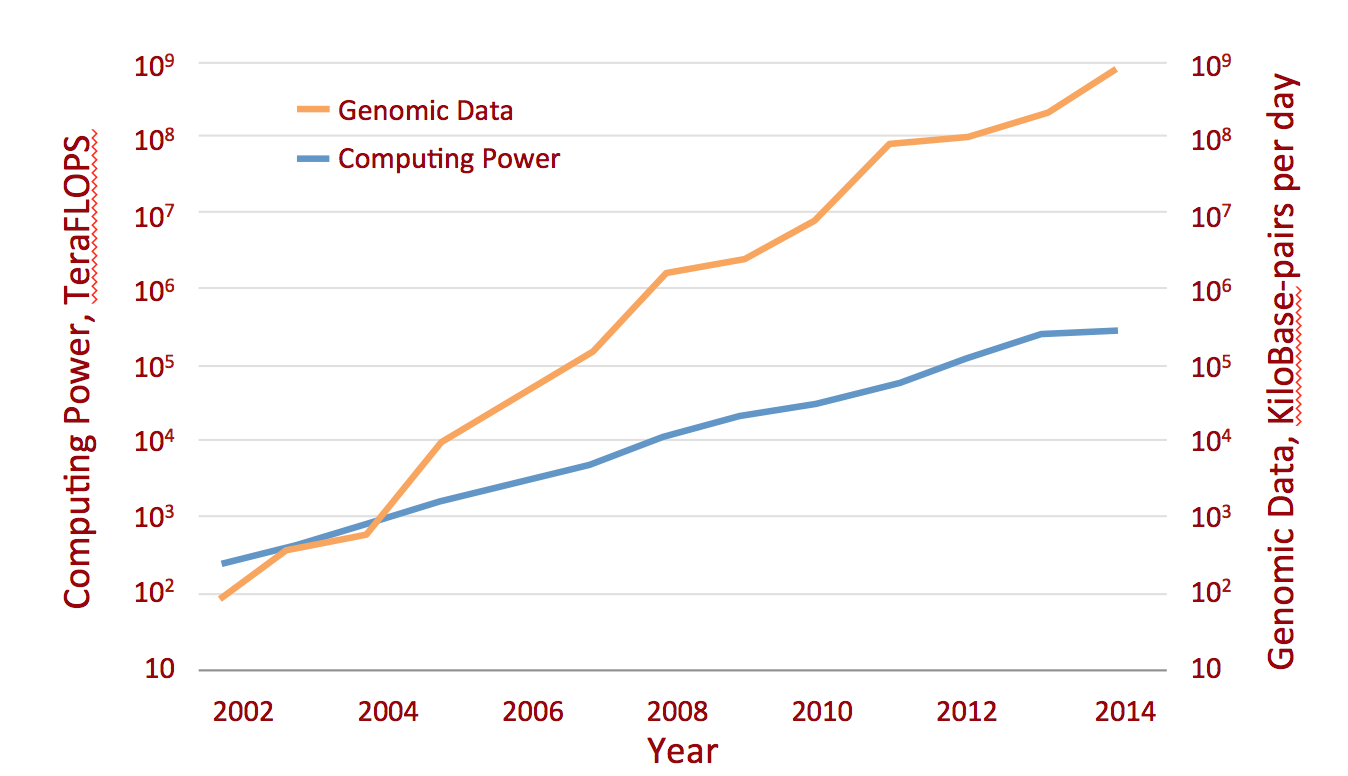
\includegraphics[width=2.8in]{assets/moore.png}
\label{fig:moore}
}
\subfloat[Growth of genomic sequence data (orange) as compared with hard drive capacity (blue); y-axis is logarithmic]{
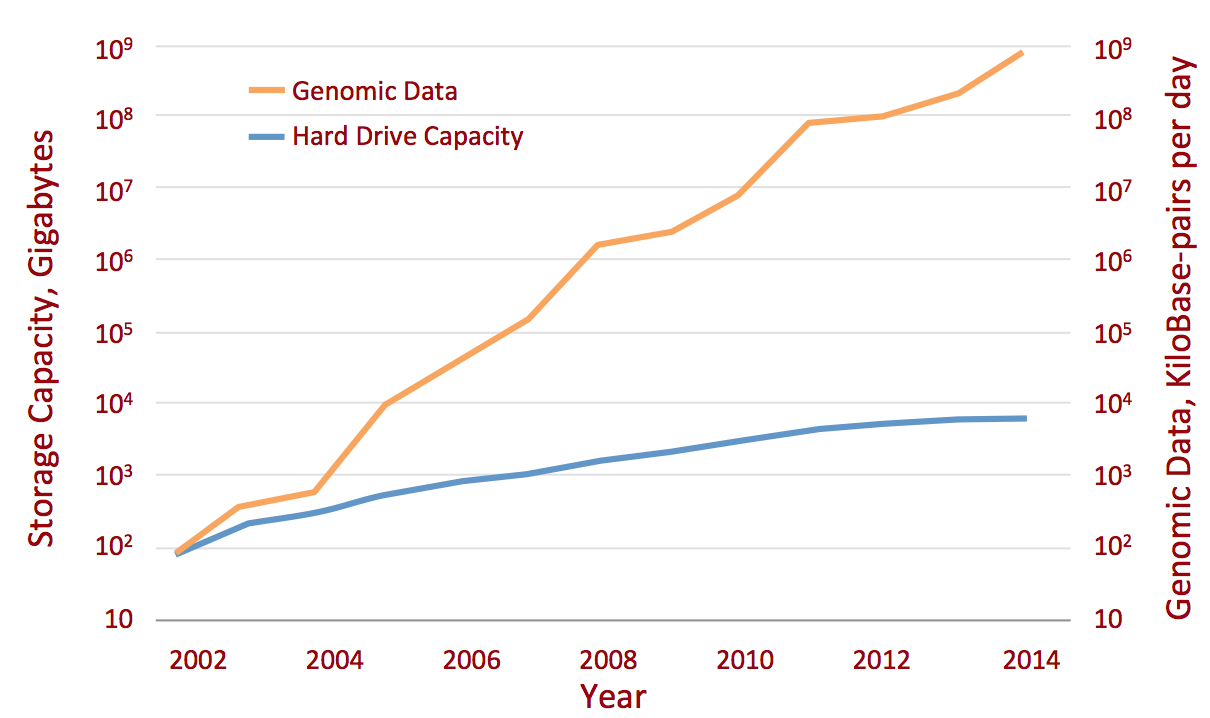
\includegraphics[width=2.8in]{assets/kryder.png}
\label{fig:kryder}
}
\caption[Sequencing vs. Storage]{Moore's (a) and Kryder's (b) laws contrasted with genomic sequence data}
\label{fig:growth}
\end{figure}

This growth in data poses significant challenges for 
researchers~\cite{marx2013biology}.
Currently, many biological 'omics` applications require us to store, access, 
and analyze large libraries of data.
One approach to solving these challenges is to embrace cloud computing.
Google, Inc. and the Broad Institute have collaborated to bring the GATK 
(Genome 
Analysis Toolkit) to the Google cloud (https://cloud.google.com/genomics/gatk).
Amazon Web Services are also commonly used for computational biology 
research and enterprise (e.g., DNANexus)~\cite{schatz2010cloud}.
However, while cloud computing frees researchers from maintaining their own
data centers, and provides cost-saving benefits when computing resources are
not needed continuously, it is no panacea.
First and foremost, cloud computing does not truly address the problem posed by
a corpus of data that is growing faster than Moore's law, because the computer
systems that make up those cloud datacenters are still themselves bound by
improvements in semiconductor technology; they still follow the trajectory
suggested by Moore's law.
Moreover, in the face of disease outbreaks such as the 2014 Ebola virus epidemic 
in West Africa, analysis resources are needed at often-remote field sites.
While it is now possible to bring sequencing equipment and limited computing 
resources to remote sites, internet connectivity is still highly constrained.
Thus, accessing cloud resources for analytics may not be possible.


Computer scientists routinely exploit the structure of various data in
order to reduce time or space complexity.
In computational biology, this approach has implicitly served researchers well.
Now-classical approaches such as principal component analysis (PCA) reduce the 
dimensionality of data in order to simplify analysis and uncover salient 
features~\cite{berger2013computational}.
As another example, clever indexing techniques such as the Burroughs-Wheeler 
Transform (BWT) take advantage of aspects of sequence 
data~\cite{berger2013computational} to speed up computation and save storage.
This review focuses on cutting-edge algorithmic advances for dealing with the growth in 
biological data by explicitly taking advantage of its unique structure; algorithms for gaining novel biological insights are not its 
focus.

\section{Types and sources of biological data}

In the central dogma of molecular biology, DNA is transcribed into RNA, which
is translated by the ribosome into a polypeptide chain, a sequence of amino 
acids, known as a protein.
This protein folds into a complex, low-energy structure, which functions as
a cellular machine; the DNA sequence determines the amino acid sequence,
which in turn determines the folded structure of the protein.
This structure ultimately determines the protein's function within the cell.
Certain kinds of RNA also function, sometimes with proteins, as cellular 
machines.
Thus, researchers are interested in DNA, RNA, and protein sequences, as well
as the structures that RNA and proteins form.
Researchers also study the resulting functions of RNA and proteins, in what
abundance they occur (gene expression), and how they interact
with each other (interaction networks).

Most but not all biological data take the form of \emph{sequence} data, either 
nucleotide sequences (nominally a four-letter alphabet representing the four 
DNA or RNA bases) or protein sequences (nominally a twenty-letter alphabet 
representing the twenty standard amino acids).
Sequence data are obtained in several ways, including mass spectrometry (which
can determine protein sequence, as well as interactions) and RNA-seq (which can determine RNA sequence, 
and by inference the expression of the gene to which it might translate).
However, the greatest volume of sequence data derive from next-generation 
sequencing (NGS) technologies, and comprise DNA sequences.
At the dawn of the genomic era, Sanger sequencing was the most widely-used 
method.
Slow and labor intensive but well-tested, Sanger sequencing is still used to 
validate NGS results.
More recently, Sanger sequencing has largely been supplanted by NGS approaches,
beginning with Illumina's ``sequencing by synthesis,'' which allows vastly 
greater throughput due to massive parallelism, low cost, and simple sample
preparation.
Importantly to this Review, Illumina sequencing, as well as other approaches
such as SOLiD, Ion Torrent, and 454 pyrosequencing, does not read a single DNA
molecule end-to-end as one could a file from a hard drive.
Instead, DNA molecules are chopped into many small fragments;
from these we can measure 
\emph{reads} from one or both ends (Figure~\ref{fig:shotgun}).
These reads are read concurrently and must be reassembled in the correct order 
if an entire genome is to be read.
Current reads most typically range from 50 to 200 bases long, though longer reads are
available with some technologies (e.g., PacBio).
This so-called ``shotgun sequencing'' is analogous to the problem of 
reconstructing a large file from small, 
randomly-ordered reads, or a shredded paper document.
However, these NGS reads overlap, and they are many in number, so 
reconstructing an entire genome is feasible.
No sequencing technology is completely infallible, so sequencing machines also
provide a \emph{quality score} (or measure of the confidence in the DNA base
called) associated with each position.
Thus, an NGS read is a string of DNA letters, coupled with a string of ASCII
characters that encode the quality of the base call.
A sequencing run will produce many of these reads, typically stored in a FASTQ
file.

Another important type of biological data is gene expression, or the quantity of
a particular gene product (usually a protein and more recently RNA) present in the cell.
Gene expression data is useful for relating genotype to phenotype, and is 
important in studying diseases including cancer.
Usually obtained through microarrays or RNA-seq technologies, expression data is
quantitative, as each gene from a sample is associated with a numeric expression
level, and high-dimensional, as many thousands of genes may be analyzed at a
time.
Resources such as NCBI’s Gene Expression Omnibus (GEO), which pool 
together many diverse expression studies, now allow researchers to analyze 
thousands of samples generated by others to obtain meaningful biological 
insights. 
More importantly, many of these biological insights can only be gleaned when 
viewed in the context of hundreds or thousands of gene expression samples.

Protein structure data, primarily determined through X-ray crystallography or
nuclear magnetic resonance (NMR) spectroscopy, describes the coordinates of 
each atom, in Angstroms, of a protein in three-dimensional space.
This information is important to understanding how a protein functions, because
proteins interact physically with other molecules.
Protein structure data are commonly stored in the Protein Data Bank (PDB); 
each PDB entry has an associated resolution indicating the accuracy of the
structural description.
Thus a PDB entry at its most basic level contains a list of atoms, along with
which amino acid they belong to and their spatial coordinates as floating-point
numbers.

Chemical compounds represent another source of structural data, more general
than proteins.
Determined by X-ray crystallography, NMR, electron microscopy and other 
techniques, compounds---many of which are useful pharmaceuticals---can be
represented as labeled graphs.
In such a graph, the vertices are atoms (labeled with a chemical element) and
the edges are bonds between atoms (labeled with a bond type, such as single or
double).
Chemical compounds are stored in databases such as PubChem, and can be described
as adjacency matrices.

Networks are frequently used to represent biological data, such as the genetic
and physical interactions among proteins, as well as those in metabolic 
pathways~\cite{berger2013computational}.

\section{Challenges with biological data}

Given DNA or RNA reads from NGS technologies, the first task is to 
\emph{assemble} those fragments of sequence (which have associated quality 
scores) into contiguous sequences.
The task of \emph{de novo} assembly is beyond the scope of this Review, but is
possible because reads overlap and because the sequence is covered by many such
overlapping reads~\cite{zhang2011practical}; the \emph{de Bruijn graph} is a 
commonly-used data structure.
Often, however, a \emph{reference genome} (or in the case of RNA, 
\emph{transcriptome}) is available for the organism being sequenced; the
establishment of a human reference genome was indeed the purpose of the Human
Genome Project.

When a reference sequence is available, NGS reads can be \emph{mapped} onto
this reference (Figure~\ref{fig:ngs-pipeline}).
Mapping allows the differences between the newly-sequenced genome and the 
reference to be analyzed; these differences, or variants, may include single-nucleotide polymorphisms
(SNPs, which are the genetic analogue to bit-flips) (Figure~\ref{fig:snps}), 
insertions or deletions, or larger-scale changes in the genome.
Determining the differences between an individual genome and a reference is
known as \emph{variant calling}.
While reference-based read mapping is a fundamentally simpler problem than
\emph{de novo} assembly, it is still computationally complex, as gigabytes or
terabytes of reads must each be mapped onto the reference genome, which can 
range from millions (for bacteria) to billions (for mammals).
As an example, the ICGC-TCGA Pan Cancer Analysis of Whole Genomes 
(PCAWG)~\cite{weinstein2013cancer} brings together more than 500 top cancer researchers from about 80 institutions in a coordinated manner with the goal of mapping the entire mutational landscape of 37 common cancer types. 
Currently each sample requires seven hours to download. 
Importantly, researchers do not trust the provided mapping, and thus they redo mappings. 
The time spent on mapping is about 50\% of the overall time spent on the sequence analysis pipeline. 
As read mapping is typically the most costly step in NGS analysis pipelines (e.g., GATK), any improvement to existing mappers will immediately accelerate sequence analysis studies on large read datasets.



\begin{figure}[htb!]
\centering
\subfloat[``Shotgun'' sequencing breaks DNA molecules into many short fragments, which are read from one or both ends in the form of {\em reads,\/} and relies on high coverage to produce a statistically likely representation of a whole genome]{
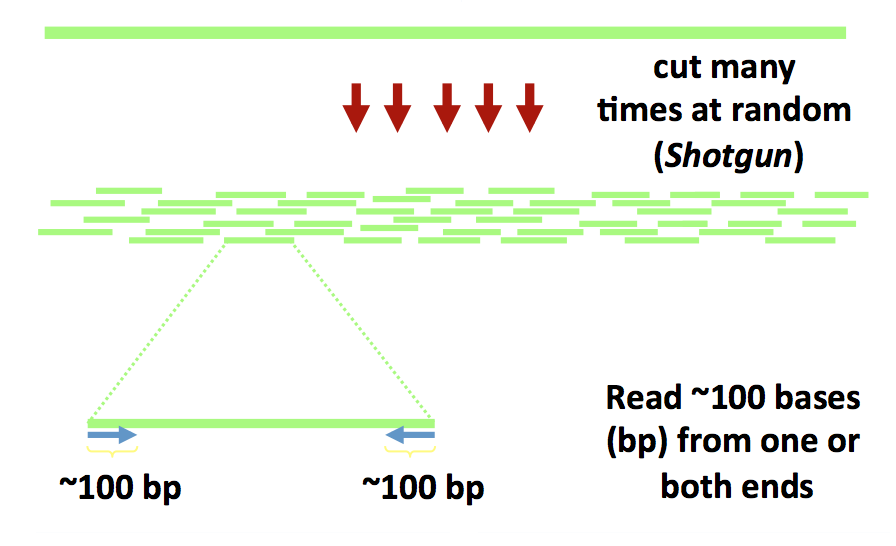
\includegraphics[width=2.6in]{assets/shotgun.png}
\label{fig:shotgun}
}
\subfloat[Single-nucleotide polymorphisms, or SNPs, are the simplest type of genomic variant, and form the bulk of ``variant-calling'' analysis]{
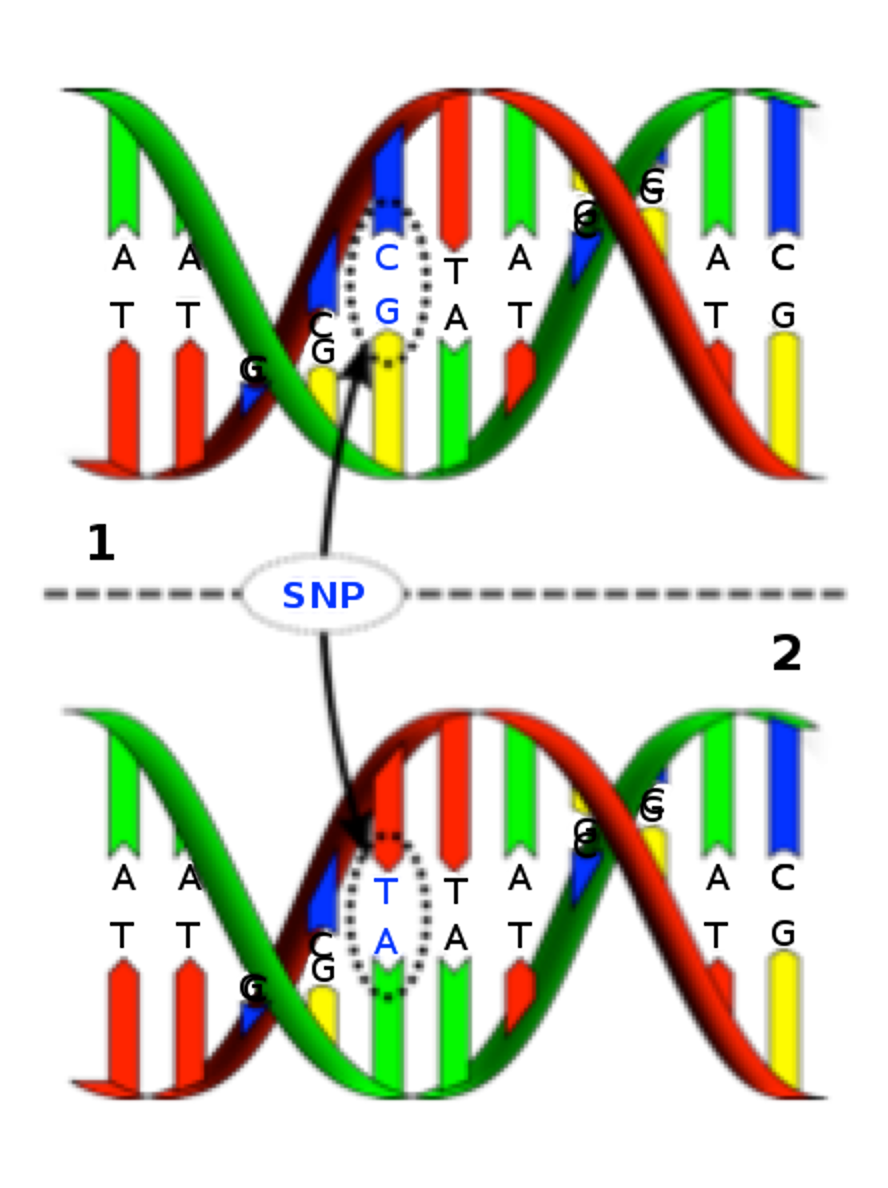
\includegraphics[width=2.6in]{assets/snps.png}
\label{fig:snps}
}\\
\subfloat[The NGS downstream analysis pipeline. Shotgun reads are mapped to a reference genome with tools such as BWA or Bowtie. The resulting genomic sequence is analyzed for variants with tools such as GATK or Samtools. This allows relationships between genes and diseases to be uncovered.]{
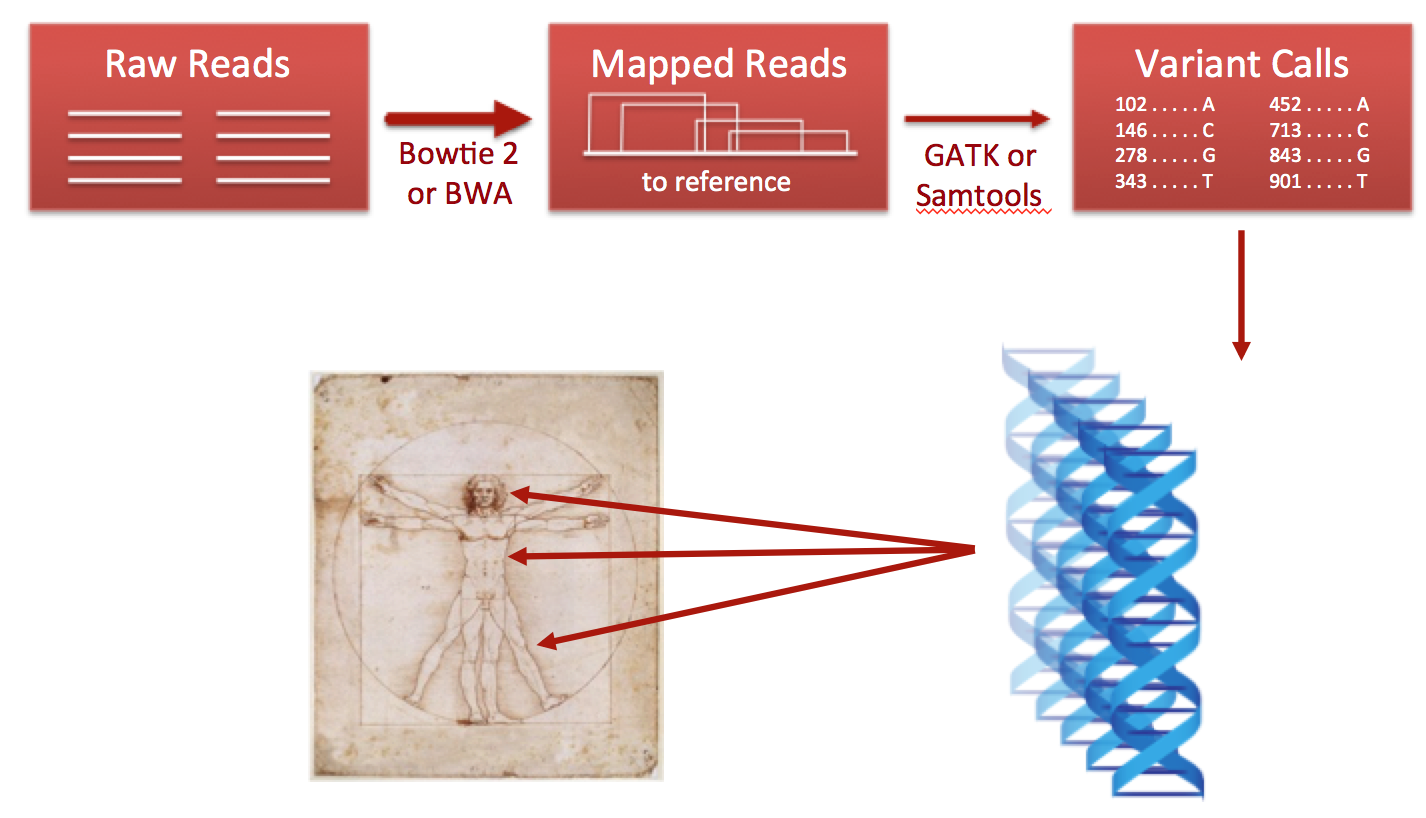
\includegraphics[width=4.0in]{assets/ngs-pipeline.png}
\label{fig:ngs-pipeline}
}
\caption[The NGS Pipeline]{The next-generation sequencing (NGS) pipeline.}
\label{fig:ngs}
\end{figure}

Driven by the plummeting costs of next-generation sequencing, the 1000 Genomes Project~\cite{10002012integrated} is pursuing a broad catalog of human 
variation; instead of producing a single reference genome for a species, many
complete genomes are catalogued.
Likewise, WormBase~\cite{harris2014wormbase} and 
FlyBase~\cite{tweedie2009flybase} are cataloguing many different species and
strains of the \emph{Caenorhabditis} worm and \emph{Drosophila} fruit fly, 
respectively.
These genomes are enabling cross-species inference, for example about genes and regulatory regions, and thus insights into function and
evolution~\cite{berger2013computational}.
Again, the sheer enormity of sequencing data is problematic for storage, access and analysis.

On a potentially even larger scale is the growth of metagenomic data.
Metagenomics is the study of the many genomes (bacterial, fungal, and even 
viral) that make up a particular environment.
Such an environment could be soil from a particular region (which can lead to 
the discovery of new 
antibiotics~\cite{gillespie2002isolation,forsberg2012shared}), or it could be 
the human gut, whose microbiome has been linked to human-health concerns 
including Autism Spectrum Disorder~\cite{macfabe2012short}, 
Crohn's Disease~\cite{gevers2014treatment,manichanh2006reduced}, and 
obesity~\cite{greenblum2012metagenomic}.
Metagenomics fundamentally asks what organisms are present, and, in the case
of a microbiome such as the gut, what metabolic functions it can accomplish as
a whole.
One way of addressing this problem is to attempt to map NGS reads from a metagenomic sample
onto a set of reference genomes that are expected to be present.
This is exactly the read-mapping problem discussed above, but with many 
reference genomes, compounding the computational requirements.
A second way is to perform homology search on a protein sequence database;
exact or nearly-exact matches imply the presence of a species, while more 
distant hits may still give clues to function.
For this task, BLASTX~\cite{altschul1990basic} is commonly
used to translate nucleotide reads into their possible protein sequences, and
search for them in a protein database.
The difficulty is that the datasets required to shine any light on these 
questions, namely from ``shotgun'' metagenomics, are gigantic and vastly more 
complex than 16S metagenomic studies that merely classify the bacteria based on 
their divergence with respect to a specific gene.
The massive data results in major identification 
challenges for certain bacterial, as well as viral, species and 
genera~\cite{janda200716s}. 

Given a sequenced genome, the next natural questions are what genes (genomic
regions that code for proteins) are present, what structure each resulting
protein takes, and what biological function it performs.
Identifying likely genes is a well-studied problem~\cite{burge1998finding} 
beyond the scope of this Review.
However, determining evolutionary relationships, structure, and function are
at the heart of current research in computational biology.
Since some organisms (known as \emph{model organisms}) are better studied than
others, and evolution is known to conserve sequence, structure, and function,
a powerful approach to determine these attributes is to search for similar
sequences about which more is known. 
This so-called \emph{homology search} entails searching for \emph{approximate}
matches in databases of known gene or protein sequences.
The homology search problem was previously believed to be solved;
Basic Local Alignment Search Tool (BLAST)~\cite{altschul1990basic} had been
the standard tool for performing homology (similarity) search on databases of nucleotide and
protein sequences.
BLAST takes a ``seed-and-extend'' approach; it looks for small, $k$-mer matches
that might lead to longer matches, and greedily extends them, ultimately 
producing a \emph{sequence alignment} between a query and each potential 
database hit.
However, BLAST's running-time scales linearly with the size of the database being
searched, which is problematic as sequence databases continue to grow at a
faster rate than Moore's law.

While gene expression data lends itself to cluster analysis and probabilistic 
approaches, the high dimensionality and noise in the data presents significant 
challenges~\cite{nguyen2002tumor}.
Principal Component Analysis has shown promise in reducing the dimensionality
of gene expression 
data~\cite{raychaudhuri2000principal,alter2000singular,yeung2001principal,misra2002interactive}.
Such data and its challenges have been the focus of other 
articles~\cite{berger2013computational}, and thus will be only lightly touched 
upon here.

Over the course of evolutionary time, structure is known to be more highly 
conserved than sequence~\cite{illergaard2009structure}, which is to say that it 
does not change as rapidly.
When the structure of a protein is known but its biological function or 
evolutionary relationships are not, researchers may search for structurally
similar proteins that are better studied~\cite{gibrat1996surprising}.
Classical tools for this involve performing pairwise structural alignments to
look for geometric similarity; DALI~\cite{holm1995dali} is still widely used,
along with other aligners such as FATCAT~\cite{ye2004fatcat} and 
Matt~\cite{menke2008matt}.
Due to the complexity of protein structures, these programs generally take 
significant amounts of time,
especially to align multiple structures.
For example, the DALI webserver can take as much as an hour to return results
for a single query.
FragBag~\cite{budowski2010fragbag} accelerates protein structure search by
approximating structural alignments
by instead comparing the ``bag-of-words'' from each structure.
Analogous to a term-frequency vector in information retrieval, this bag-of-words
indicates the abundance of particular, short structural motifs within a protein.

The computational study of drugs and their targets based on chemical structure and function
is known as chemogenomics~\cite{bredel2004chemogenomics}.
In the fields of drug discovery and drug repurposing, the prediction 
of biologically active compounds is an important task. 
Computational high-throughput screening eliminates many compounds from 
laborious wet-lab consideration, but even computational screening can be 
time-consuming.
Chemogenomics typically relies on comparing chemical graph structures to identify
similar molecules and binding sites.
Furthermore, comparing chemical graph structures typically involves computing
the maximal common subgraph (MCS), an NP-hard problem.
However, there are once again an increasing number of such chemical compounds
to search; the NCBI's PubChem database has grown from 31 million compounds in
January 2011 to 68 million in July, 2015.

With biological networks, challenges lie in integrating such data in order to 
deduce gene function, as well as uncover disease and metabolic pathways.
Several approaches have taken advantage of the particular topologies of 
biological
networks, such as diffusion-based approaches, which explore the topology of
networks through random walks.
In protein interaction networks, some nodes are high-degree \emph{hubs,} which 
interact with
many partners; these interactions do not imply shared function as strongly as
non-hub interactions; such information needs to be teased apart.
As new functional annotations and interactions are discovered,
the number and size of these networks grows, making related problems more 
intractable~\cite{berger2013computational}.

The continued ability to store, search, and analyze these growing data sets hinges on
clever algorithms that take advantage of the structure of, and redundancy 
present in, the data.
Indeed, these growing data sets ``threaten to make the arising problems 
computationally infeasible.''~\cite{berger2013computational}

\section{State-of-the-art approaches to meet these challenges}

Techniques for reference-based read mapping typically rely on algorithmic 
approaches such as the Burrows-Wheeler transform (BWT)~\cite{burrows1994block}, 
which provides efficient string 
compression through a reversible transformation, while the FM-index data 
structure~\cite{ferragina2000opportunistic} is a compressed substring index, 
based on the BWT, which provides efficient storage as well as fast search.
BWA (Burrows-Wheeler Aligner)~\cite{li2009fast} uses the BWT, while the 
Bowtie2~\cite{langmead2012fast} mapper further relies on the FM-index for 
efficient mapping of NGS reads.
The Genome Multitool (GEM) mapper~\cite{marco2012gem} also uses an FM-index 
coupled with dynamic programming in a compressed representation of the 
reference genome, in order to prune the search space 
when mapping reads to a reference genome.
Masai~\cite{siragusa2013fast} and mrsFAST \cite{hach2014mrsfast} use an ``approximate seed'' approach to indexing
the space of possible matches, likewise pruning the search space; however, the
bulk of its runtime is spent on the extend phase.
State-of-the-art mapper mrsFAST-Ultra achieves improvements in efficiency based on machine architecture rather than leveraging redundancy in the data itself with near-perfect sensitivity, but
only for the case where there are no insertions and deletions (indels) \cite{hach2014mrsfast}.
Even with these approaches, read mapping remains a significant bottleneck in
genomic research~\cite{hach2010mrsfast}.

Recent advances in metagenomic search tools have relied on two improvements over
BLASTX: indexing and alphabet reduction.
RapSearch2~\cite{zhao2012rapsearch2} relies on alphabet reduction and a 
collision-free hash table.
The alphabet reduction, as it is reversible, can be thought of as a form of
lossless compression; a 20-letter amino acid alphabet is mapped onto a smaller
alphabet, with offsets stored to recover the original sequence in the full
alphabet.
The hash-table provides an efficient index of the database to be searched.
DIAMOND~\cite{buchfink2014fast} also relies on alphabet reduction, but uses
``shaped seeds'' instead of simple $k$-mer seeds to index the database.
DIAMOND demonstrates search performance three to four orders of magnitude faster
than BLASTX, but it is still linear in the size of the database being searched.

Recent work on gene expession has explored additional ways to exploit the high-dimensional 
structure of the data.
SPARCLE (SPArse ReCovery of Linear combinations of Expression)~\cite{prat2011recovering}
brings ideas from compressed sensing~\cite{candes2005decoding,candes2006stable,donoho2006compressed} 
to gene expression analysis.
Specifically, SPARCLE relies on the idea that a randomly-chosen set of points 
are unlikely to be close in a lower-dimensional linear subspace.
Thus, SPARCLE approximates a gene's expression profile as a linear combination
of a few other genes' profiles, and then applies supervised learning to
predict relationships between genes.
Another recent and novel approach to exploiting the structure of gene expression
space is Parti (Pareto task inference)~\cite{hart2015inferring}, which describes a set of
data as a polytope, and infers the specific tasks represented by vertices of
that polytope from the features most highly enriched at those vertices.
In human breast tumors, and in mouse tissues, the expression data were
well-described by tetrahedra whose vertices were enriched for different tumor
types and biological functions, from which four distinct tasks are 
inferred~\cite{hart2015inferring}.

The most widely-used chemogenomics search is the Small Molecule Subgraph Detector 
(SMSD)~\cite{rahman2009small}, which applies one of several MCS algorithms based
on the size and complexity of the graphs in question.
Notably, large chemical compound databases, such as PubCHEM,
cannnot be searched on a laptop computer with current tools such as SMSD.

An area of great interest in integrating biological network data is in global multiple network 
alignment, which is based on network topology and conserved biological function (IsoRank~\cite{singh2008global} and IsoRankN~\cite{liao2009isorankn}).
IsoRank's approach is similar to the PageRank algorithm~\cite{page1999pagerank} 
but performs a random walk on the product graph of two networks;
IsoRankN produces a \emph{Personalized PageRank} alignment, similar to the
PageRank-Nibble algorithm~\cite{andersen2006local}.
Diffusion state distance (DSD)~\cite{cao2013going} is a diffusion-based approach
which defines a distance metric between two nodes based on random walks.
DSD penalizes high-degree nodes, and outperforms other graph-theoretic distance
functions when applied to standard approaches such as neighbor voting for function annotation.
Diffusion component analysis (DCA)~\cite{cho2015diffusion} amounts to a network-based 
analogue of principle component analysis; DCA reduces the dimensionality of a
network in such a way that function annotation can be performed in the reduced 
space, significantly decreasing running time while still providing competitive
prediction accuracy.
Using a compressed representation of metabolic networks, 
Mongoose~\cite{chindelevitch2014exact} is able to 
identify and unblock many blocked reactions in current models without loss of 
accuracy.


\section{Structure of biological data}\label{structure}

Fortunately, biological data has unique structure \cite{yu2015entropy}, which we 
will take advantage of to perform search that scales sublinearly in the size of the database~(Section~\ref{omics}).
The first critical observation is that
much biological data is highly redundant; if a computation is performed on one
human genome, and a researcher wishes to perform the same computation on another
human genome, most of the work has already been done \cite{loh2012compressive}.
When dealing with redundant data, clustering comes to mind.
While cluster-based search is well-studied~\cite{jardine1971use}, conventional
wisdom holds that it provides a constant factor speed-up over exhaustive search.

Beyond redundancy, however, another attribute of large biological data sets
stands out.
Any high-dimensional data set, such as amino acid sequences of a bounded 
length, can be described as inhabiting a vector space.
For example, given an alphabet of 20 amino acids and a length bounded at 
500\footnote{While the largest-known protein, titin, is over 33,000 amino acids 
in length, proteins are typically described as comprising \emph{domains} that 
evolve and fold independently; domains rarely exceed 500 amino acids.}, one 
could
enumerate $20^{500} \approx 3 \times 10^{650}$ distinct protein sequences, as 
of July 
2015, the NCBI's exhaustive ``NR'' database lists $6.9 \times 10^{7}$ sequences.
This surprisingly lower number is not simply due to undersampling; thanks to 
evolution, only those protein
sequences which exhibit useful biological function should survive, and most
random sequences of amino acids would not be expected to form stable structures.
Thus, not only do biological data exhibit redundancy, they also tend not to 
inhabit anywhere near the entire feasible space (Figure~\ref{fig:clusters}).
It seems that physical laws have constrained the data to a particular subspace
of the enumerable Cartesian space.

\begin{figure}[htb!]
\centering
\subfloat[Cartoon depiction of points in an arbitrary high-dimensional space, 
as might arise from genomes generated by mutation and selection during the 
course of evolution. 
Although high-dimensional locally, at the global scale of covering spheres, the 
data cloud looks nearly 1-dimensional, which enables entropy-scaling of 
similarity search. Clusters cover the data points but do not cover unoccupied 
regions of space.]{
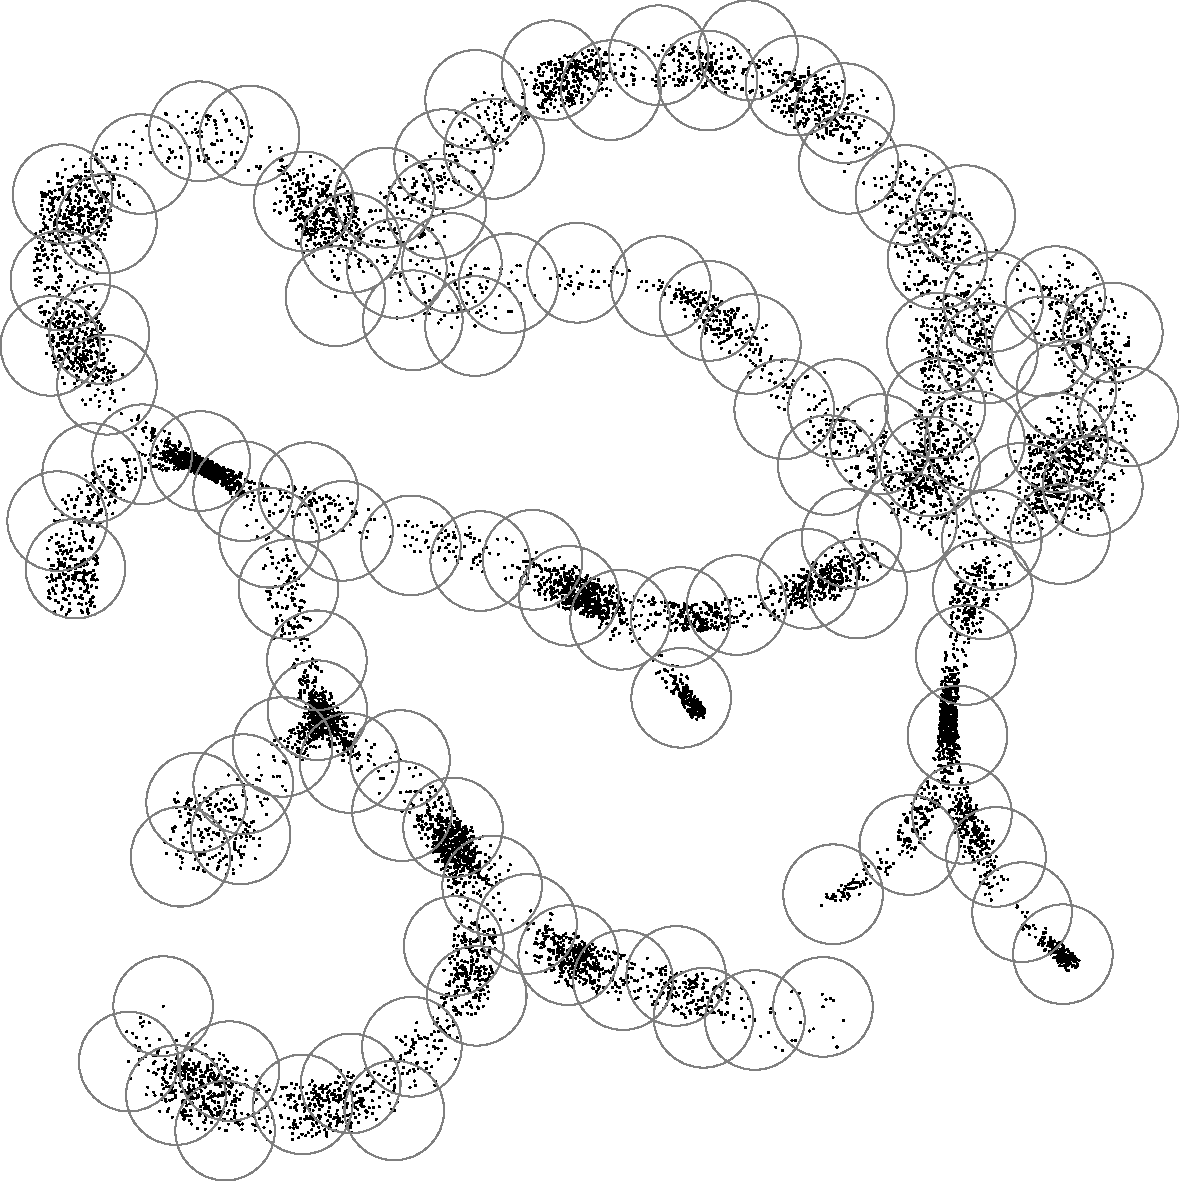
\includegraphics[width=2.8in]{assets/treepoints.pdf}
\label{fig:clusters}
}
\subfloat[A query (green triangle) and two concentric search radii (red 
circles) around it. Thanks to low fractal dimension, the large circle does
not contain vastly more points than the small circle.]{
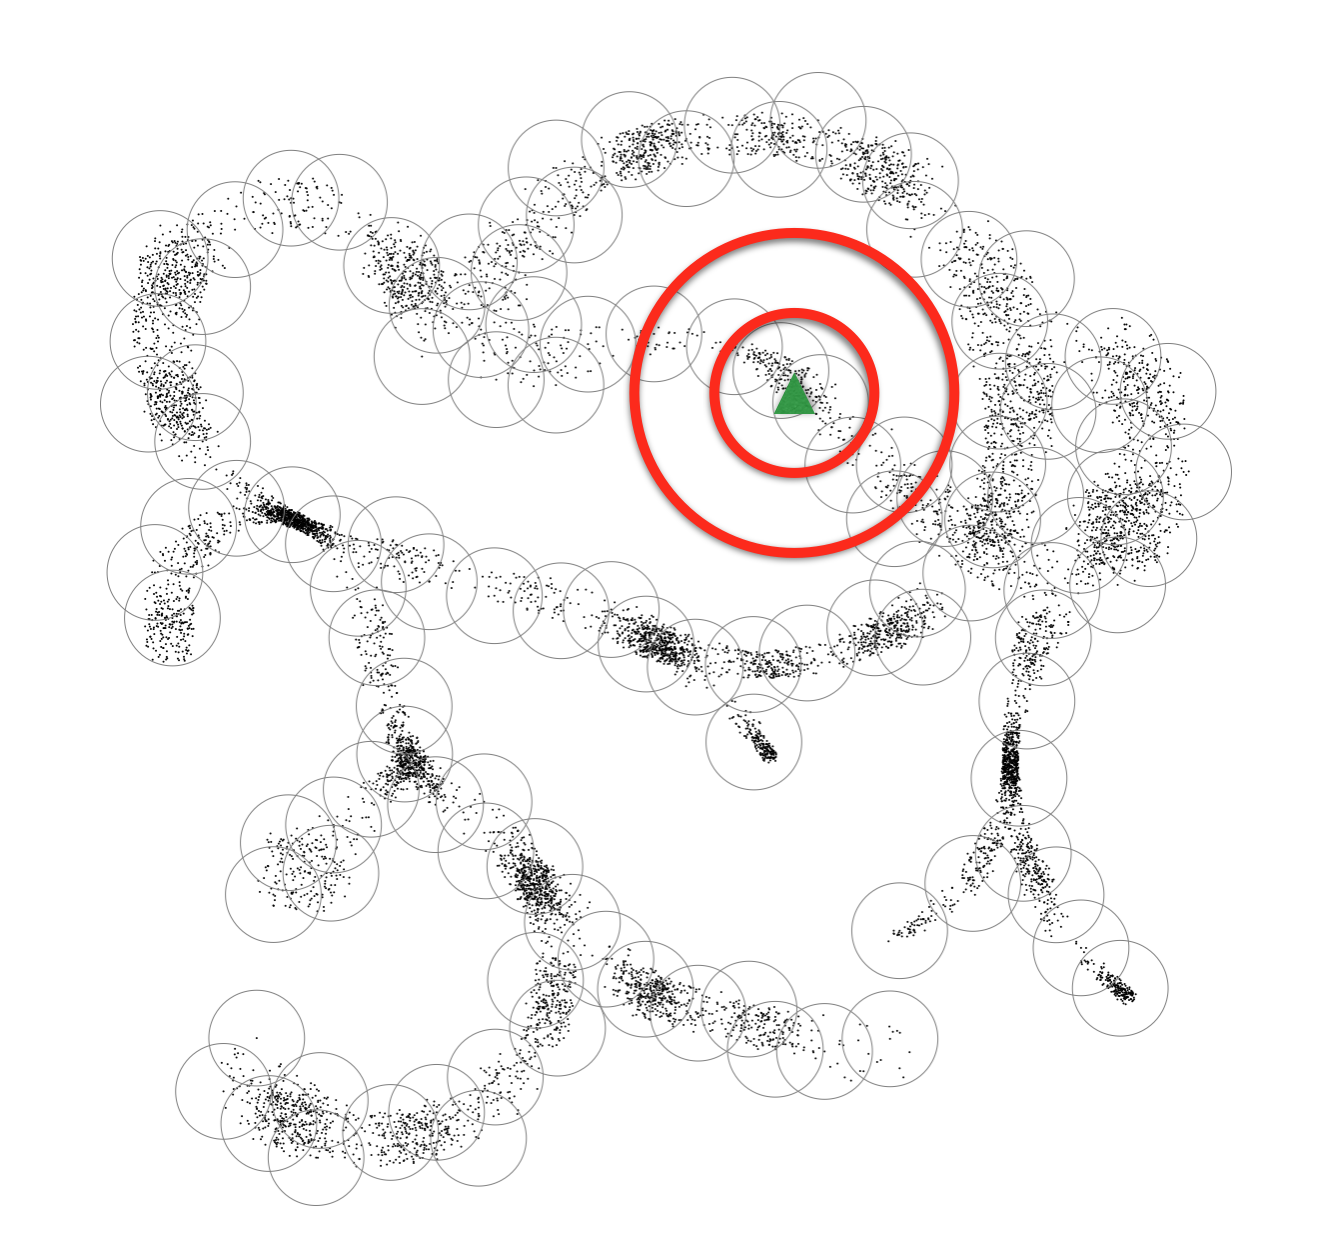
\includegraphics[width=2.8in]{assets/treepoints-fractal.png}
\label{fig:fractal}
}
\caption[Data spaces.]{A cartoon illustration of a biological data space.}
\label{fig:dataspace}
\end{figure}

One key insight related to redundancy
%as to why the compressive omics approach allows computation 
%that scales sublinearly in the size of the data 
is that such data sets exhibit
low \emph{metric entropy}~\cite{yu2015entropy}.
That is, for a given cluster radius $r_c$ and a database $D$, the number $k$ 
of clusters needed to cover $D$ is bounded by $N_{r_c} (D)$, the metric 
entropy, which is relatively small compared to
$|D|$, the number of entries in the database (Figure~\ref{fig:clusters}).
In contrast, if the points were uniformly distributed about the Cartesian space,
$N_{r_c} (D)$ would be larger.

A second key insight is that the biological data sets have low \emph{fractal dimension}~\cite{yu2015entropy}.
That is, within some range of radii $r_1$ and $r_2$ about an arbitrary point
in the database $D$, the fractal dimension $d$ is
$d=\frac{\log (n_2 / n_1)}{ \log (r_2 / r_1)}$, where $n_1$ and $n_2$ are the
number of points within $r_1$ and $r_2$ respectively (Figure~\ref{fig:fractal}).

Cluster-based search, as exemplified by ``compressive omics,'' can perform
approximate search within a radius $r$ of a query $q$ on a database $D$ with 
fractal dimension $d$ and metric entropy $k$ at the scale $r_c$ in time
proportional to
\[
    O\Bigg(
    \underbrace{k}_{\textrm{metric entropy}} +
    \overbrace{\left|B_D(q,r)\right|}^{\textrm{output size}}
    \underbrace{\left(\frac{r+2r_c}{r}\right)^d}_{\textrm{scaling factor}}
     \Bigg) .
\]

Given this formalization, the ratio $\frac{|D|}{k}$ provides an estimate of the 
speed-up factor for the coarse search component compared to a full linear 
search.
The time-complexity of the fine search is exponential in the fractal dimension
$d$, which can be estimated globally by sampling the local fractal dimension 
over a dataset.
Table~\ref{fractal} provides the fractal dimension $d$ sampled at typical query
radii, as well as the ratio $\frac{|D|}{k}$, for nucleotide sequence, protein 
sequence, protein structure, and chemical compound databases.

Biological data sets exhibit redundancy, and are constrained to subspaces by
physical laws.
This combination results in low fractal dimension and low metric entropy 
relative to the size of the data set, which suggests that ``compressive omics''
will provide the ability for computation to scale sublinearly with massively growing data.

\begin{table}
\label{fractal}
\caption{Metric entropy ratio (ratio of clusters to entries in database) and
fractal dimension at typical search radii for four biological data sets.
NCBI's ``NR'' non-redundant protein sequence and ``NT'' non-redundant nucleotide sequence databases are from June, 2015. Protein Databank (PDB) is from July, 2015. PubChem is from October, 2013.}
\begin{tabular}{ccc}
\hline
Data set & Metric entropy ratio & Fractal dimension \\        
\hline
Nucleotide sequences (NCBI NT) & 7:1 & 1.5\\
\hline
Protein sequences (NCBI NR) & 5:1 & 1.6\\
\hline
Protein structure (PDB) & 10:1 & 2.5\\
\hline
Chemical structure (PubChem) & 11:1 & 0.2\\
\hline
\end{tabular}
\end{table}

\section{The age of compressive omics}\label{omics}

We are entering the age of compressive omics, 
which makes use of this completely different paradigm for the structure of biological data.
Seeking to take advantage of the redundancy inherent in genomic sequence data, 
Loh, Baym and Berger \cite{loh2012compressive}
introduced \emph{compressive genomics}, an approach that relies on compressing
data in such a way that the desired computation (such as BLAST search) can be
performed in the compressed representation.
Daniels et al. \cite{daniels2013compressive} further demonstrated that
compressive acceleration takes advantage of increasing redundancy in the
data over time.

Compressive genomics is based on the concept of \emph{compressive acceleration},
which relies on a two-stage search, referred to as \emph{coarse} and \emph{fine} search.
Coarse search is performed only on the coarse, or representative, subsequences
that represent unique data.
Any representative sequence that is within some threshold of the query is then expanded 
into all the similar sequences it represents; the fine search is then over this
(typically small) subset of the original database.
This approach provides orders-of-magnitude run-time improvements to BLAST search on 
nucleotide~\cite{loh2012compressive} and protein~\cite{daniels2013compressive}
data; moreover, these run-time improvements increase as databases grow.

The CORA read mapper~\cite{yorukoglu2015compressive} applies a mid-size $l$-mer based 
read-compression approach with a compressive indexing of the reference genome
(referred to as a homology table).
CORA, like caBLAST and caBLASTP, accelerates existing tools (in this case, read
mappers including BWA or Bowtie2) by allowing them to operate in a compressed
space, and relying on a coarse and a fine phase.
In contrast, short seed-clustering schemes, such as those used in Masai~\cite{siragusa2013fast} and 
MrsFAST~\cite{hach2010mrsfast}, conceptually differ from CORA in that those 
schemes aim to accelerate only the seed-to-reference matching step.
Thus, there is a subsequent seed-extension step, which is substantially more 
costly and still needs to be performed for each read and mapping individually, 
even when seeds are clustered. 
Through its $l$-mer based read compression model, CORA is able to accelerate 
and 
achieve asymptotically sublinear scaling for both the seed-matching and 
seed-extension steps within coarse-mapping, which comprises the major bulk of 
the read-mapping computation.
Traditionally, $k$-mers refer to short substrings of fixed length (often, but 
not necessarily, a power of two) used as ``seeds'' for longer sequence matches.
CORA uses much longer $k$-mers (e.g., 33-64 nucleotides long), and links each one to its neighbors within
a small Hamming or Levenshtein distance.
The term $l$-mer distinguishes these substrings from typically-short $k$-mers.

In the area of metagenomic search,
the recently-released MICA~\cite{yu2015entropy} demonstrates that the 
compressive-acceleration approach of 
caBLAST~\cite{loh2012compressive} and caBLASTP~\cite{daniels2013compressive} is 
largely orthogonal to alphabet-reduction and indexing approaches.
MICA applies the compressive-acceleration framework to the
state-of-the-art DIAMOND~\cite{buchfink2014fast}, using it
for its ``coarse search'' phase and a user's choice of DIAMOND or BLASTX for its
``fine search'' phase; MICA demonstrates nearly order-of-magnitude run-time gains over the highly-optimized DIAMOND, comparable to that of caBLASTP over BLASTP.

Compressive genomics \cite{loh2012compressive} has been
generalized and adapted to non-sequence spaces as well, and coined
``compressive omics''~\cite{yu2015entropy}.
One such example is chemogenomics.
Applying a compressive acceleration approach, Ammolite~\cite{yu2015entropy}
accelerates SMSD search by an average of 150x on the PubChem database.
Another example is 
esFragBag~\cite{yu2015entropy}, which clusters proteins based on the cosine distance or
Euclidean distance of their bag-of-words vectors, further accelerating FragBag's
running time by an average of 10x.

\section{Storage compression}

Along with a genome sequence, modern sequencing systems provide a measure of
the quality of, or confidence in, the nucleotide base read at every position.
While nucleotides reside in a 4-letter alphabet, na\"ively representable in two 
bits per position, these quality scores occupy a larger range, na\"ively
requiring six or seven bits per position.
Thus, quality scores offer low-hanging fruit with respect to compression for 
storage and transmission of sequence data.
Several approaches to compressing quality scores have been 
presented~\cite{janin2013adaptive,bonfield2013compression,ochoa2013qualcomp,yu2015quality,yu2014traversing}.
Quartz~\cite{yu2015quality} takes the unusual approach of applying lossy 
compression, by bounding the likelihood that a quality score is informative.
Importantly, Quartz modifies the FASTQ file of the reads and quality scores, and thus can be
readily incorporated into existing sequence analysis pipelines.
Surprisingly, Quartz not only demonstrates improved compression over competing
approaches, but slightly improves the accuracy of downstream variant-calling.

Also taking advantage of sequence redundancy, Mince~\cite{patro2015data} groups 
similar reads (those that share a common 
substring) together into ``buckets'', allowing that common substring to now be 
removed and treated as the bucket label, so that each read in the compressed 
representation comprises only its unique differences from the bucket label.
This approach allows a general-purpose compressor to achieve tight compression.
SCALCE~\cite{hach2012scalce} also relies on a ``boosting'' scheme, reordering
reads in such a way that a general-purpose compressor achieves improved
compression ratios.



% In the realm of protein structure prediction, it has been
% observed~\cite{dunbrack2002rotamer} that rather than exploring the continuous
% range of
% possible dihedral angles, protein structures inhabit a smaller subspace, defined
% by a narrower range of angles, referred to as
% rotamers~\cite{dunbrack1993backbone}.
% The TreePack algorithm~\cite{xu2006fast} takes advantage of this observation
% for the
% purpose of sidechain packing (finding the lowest-energy conformation for the
% sidechain of each amino acid), using tree width to reduce the search space and
% simplify dependencies.



\section{Conclusions and future prospects}

The explosion of biological data, largely due to technological advances such as
next-generation sequencing, presents us with challenges as well as 
opportunities.
The promise of unlocking the secrets of diseases such as cancer, obesity,
Alzheimer's, autism spectrum disorder, and many others, as well as better 
understanding the basic science of biology, relies on researchers' ability to 
analyze the growing flood of genomic, metagenomic, structural, and interactome 
data.

The approach of compressive acceleration~\cite{loh2012compressive}, and its 
demonstrated ability to scale with the metric entropy of the 
data~\cite{yu2015entropy}, while providing orthogonal benefits to many other
useful indexing techniques, is an important tool for coping with the deluge of
data.
The extension of this compressive acceleration approach to 
metagenomics~\cite{yu2015entropy}, NGS read 
mapping and chemogenomics~\cite{yorukoglu2015compressive} suggests its 
flexibility.

The field of computational biology must continue to innovate, but also to 
incorporate the best ideas from other areas of computer science.
For example, the compressive-acceleration approach bears similarity to a metric 
ball tree, first described in the database community over twenty years 
ago~\cite{uhlmann1991satisfying};
however, the latter does not allow one to analyze performance guarantees, 
in terms of metric entropy and fractal dimension.
Other ideas from image processing, computational geometry, sublinear-time algorithms~\cite{rubinfeld2011sublinear}, and other areas 
outside of biology are likely to bear fruit~\cite{indyk1998approximate}. 
In turn, it is also likely that algorithmic ideas developed within computational biology
will become useful in other fields experiencing a data deluge, such as astronomy
or social networks~\cite{stephens2015big}.


While this Review has focused on the importance of algorithms that leverage the
structure of data to cope with the increased throughput in computational 
biology, it is also essential that techniques continue to make better 
predictions and models that demonstrate improved fidelity to wet-lab 
experiments.

\section{Acknowledgments}





% Bibliography
\bibliographystyle{ACM-Reference-Format-Journals}
% \bibliographystyle{abbrv}
\bibliography{main}



\end{document}
% End of v2-acmsmall-sample.tex (March 2012) - Gerry Murray, ACM


